\documentclass{SSBT-BE}
\usepackage{makeidx}
\usepackage{amssymb}
\usepackage{amsmath}
\usepackage{subfigure}
\usepackage{%
  babel,
  algorithmic,
  algorithm,
  caption
}

\usepackage{url}
\usepackage[breaklinks=true]{hyperref}

\usepackage[intoc]{nomencl}
\renewcommand{\nomname}{Abbreviations}
\makenomenclature
\usepackage{imakeidx}
\makeindex

\begin{document}

\title{House Price Prediction Using Machine Learning}
\author{Janhavi Kailas Chaudhari \\ Anup Sanjay Patil \\ Mayur Manohar Patil \\ Bhushan Ramkrushna Upasani \\ Priyakumari Kailassing Rajput }

\dept{Department of Computer Engineering}
\supervisor{Miss. Priti Sharma}
\submitdate{2020 - 2021}
\degree{Bachelor of Engineering}
\specialization{Computer Engineering}
\type{Project}
%\type{Seminar}
\hod{Prof. Dr. Girish K. Patnaik}

\beforepreface


\prefacesection{Acknowledgements}
%\input{acknowledgement}
We take the opportunity to express our gratitude to all those who have rendered co-operation
and guidance that supported us while analyzing and developing the design of this project
right from beginning up till now.
First of all we would like to express our deepest appreciation toward Dr. Girish K. Patnaik
(H.O.D. of Computer Engineering) and Miss. Priti Sharma (Guide) whose valuable guidance
supported us in completing the analysis and designing of our final year project. We would also like to
thank and express our respect and gratitude to Dr. K. S. Wani (Principal) for providing
us this opportunity.
Last but not least we are profoundly grateful and obliged to Miss. Priti Sharma, for her guidance, motivation and continuous encouragement throughout to see that
whole process is right on its target since its commencement.


\acknowledgeauthor



% Use following command at the command prompt to display the Abbreviations
% makeindex thesis.nlo -s nomencl.ist -o thesis.nls
\newpage
% \addcontentsline{toc}{chapter}{List of Abbreviations}
% \printnomenclature


\newpage
\afterpreface
\listoftables
\listoffigures
%\input{glossary}
\clearpage
\pagenumbering{arabic}
\pagestyle{plain}


\prefacesection{Abstract}
Machine learning plays a major role from past years in image detection, spam reorganization, normal speech command, product recommendation and medical diagnosis.
Present machine learning algorithm helps in enhancing security alerts, ensuring public safety and improve medical enhancements. Machine learning system also provides
better customer service and safer automobile systems.\\
Designing an effective machine learning model for prediction of regression and classification problem is a tedious endeavor. Significant time and expertise are needed to
customize the model for a specific problem. A significant way to reduce the complicated design is by using Automated Machine Learning (AML) that can intelligently
optimize the best pipeline suitable for a problem or dataset. This study utilizes machine learning algorithms as a research method that develops housing price prediction
models. In that point a housing cost prediction model to support a house vendor or a
real estate agent for better information based on the valuation of house is recommended.

% \chapter{Introduction}
% 
Proposed system aims to make a machine learning model which could predict the real estate house prices. Respective chapter has in view of the content focusing on scope, motivation, objectives and selection of life cycle model of the projected system. It also states the actual problem definition which is to be solved using machine learning models .\\
The Section 1.1 describes the background of the promised proposed system to be built. Motivation behind selecting particular problem statement is presented in section 1.2. The section 1.3 discuss about the problem definition. The scope of the system is discussed in section 1.4. The section 1.5 discuss about objectives of proposed system. The selection of life cycle model for development of system is discussed in section 1.6. The section 1.7 will discuss about organization of report. Finally, the summary is presented in the last section.

\section{Background}
% Content inside the background section

\section{Motivation}
% Content inside the motivation goes here
Being extremely interested in everything having a relation with the Machine Learning, the final year project was a great occasion to devote time to learn and confirm the interest for this field. The fact that machine learning can make estimations, predictions and give the ability for machines to learn by themselves is both powerful and limitless in terms of application possibilities.\\
Machine learning can be used in finance, medicine, almost everywhere. Hence that is the pivotal motivation of carrying out the final year project around machine learning domain.




\section{Problem Definition}
% Content of the problem definition goes here
In India, there are multiple real estate classified websites where properties are listed for sell/ buy/ rent purposes such as 99acres, housing, commonfloor, magicbricks and more. However, in each of these websites we can see lot of inconsistencies in terms of pricing of an apartment and there are some cases when similar apartments are priced differently and thus there is lot of in-transparency. Sometimes the consumers may feel the pricing is not justified for a particular listed
apartment but there no way to confirm that either. Proper and justified prices of properties can bring in a lot of transparency and trust back to the real estate industry, which is very important as for most consumers especially in India the transaction prices are quite high and addressing this issue will help both the customers and the real estate industry in the long run. We propose to use machine learning and artificial intelligence techniques to develop an algorithm that can predict housing prices based on certain input features.\\
The business application of this algorithm is that classified websites can directly use this algorithm to predict prices of new properties that are going to be listed by taking some input variables and predicting the correct and justified price i.e. avoid taking price inputs from customers and thus not letting any error creeping in the system. This study on proactive pricing of houses in the Indian context has never been reported earlier in the literature to the best of our knowledge.\\
However, the problem of house price prediction is quite old and there have been many studies and competitions addressing the same including the classic Boston housing price challenge on Kaggle. As far as housing price prediction in Indian context is concerned, use of machine learning algorithm can really get the job done.




\section{Scope}
\section{Objective}

\section{Selection of Life Cycle Model for Development}
% Content inside the selection of life cycle model

In order to accomplish the stated objective, Agile model is selected as software development life cycle model. The incentive behind selecting Agile model is because requirements
are stated clearly but the machine learning model needs to be trained and tested for better prediction on unseen data which makes the implementation and testing phase repetitive.
\begin{figure}[!ht]
\centering
        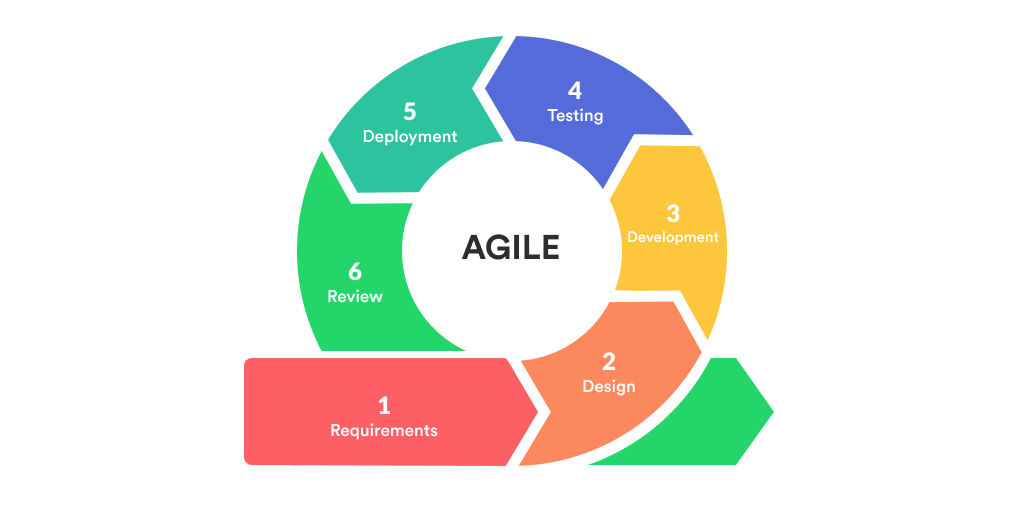
\includegraphics[totalheight=8cm]{Introduction/AgileModel.png}
    \caption{Software Development Life Cycle Model}
    \label{fig:verticalcell}
\end{figure}


\section{Organization of Report}
% Content inside the organization of the report goes here

Chapter 1: Chapter 1, Problem definition of the proposed machine learning model is given along with background history, motivation for developing this system. Scope and objective of projected system is discussed.\\ 
Chapter 2: Chapter 2, will talk about literature referred for getting this idea of project design. Actual working and functionalities of the proposed machine learning model is described here. Section 2.1 will be brief about economical, operational and technical feasibility of the given system. Risk analysis is done in section 2.2 along with planning and effort allocation for development of proposed system in section 2.3 and 2.4.\\
Chapter 3: Chapter 3, will discuss about requirements of machine learning model. Hardware as well as software requirements are described in section 3.1 and section 3.2. Section 3.3 will give functional and non functional requirements of the the model. And software requirements specification is stated in section 3.4.\\
Chapter 4: Chapter 4 will give pictorial representation of the system. Section 4.1 will show architecture of the machine learning model using simple block diagram. Section 4.2 will give data flow diagrams (DFDs). UML diagrams of the proposed system are given in section 4.3.\\
Chapter 5: In chapter 5, conclusion about whatever work had done is discussed in section 5.1. Future work are discussed in section 5.2. At the last, project report embody bibliography too.


\section{Summary}
% Content of the summary section goes here
The given chapter thoroughly describes background and motivation behind selecting this machine learning project. The problem definition, scope and objective are also stated in the given chapter. The organization of report gave the overall structure about the chapters described throughout in this report upfront. The next chapter will discuss about system analysis.


% \chapter{LaTex Basic Blocks}
% \input{./trust/gkp}

% %\chapter{Key Management}
% \label{CH-Key Management}
% %\input{./key/gkp}

% \chapter{Conclusion and Future Work}
% %\section{Conclusion}
\section{Future Work}

% \appendix
% %\input{appendix}

% \chapter{Disasters in India}
% %\input{./appendix_disaster}





%......Main Project report starts form here......

\chapter{Introduction}

Proposed system aims to make a machine learning model which could predict the real estate house prices. Respective chapter has in view of the content focusing on scope, motivation, objectives and selection of life cycle model of the projected system. It also states the actual problem definition which is to be solved using machine learning models .\\
The Section 1.1 describes the background of the promised proposed system to be built. Motivation behind selecting particular problem statement is presented in section 1.2. The section 1.3 discuss about the problem definition. The scope of the system is discussed in section 1.4. The section 1.5 discuss about objectives of proposed system. The selection of life cycle model for development of system is discussed in section 1.6. The section 1.7 will discuss about organization of report. Finally, the summary is presented in the last section.

\section{Background}
% Content inside the background section

\section{Motivation}
% Content inside the motivation goes here
Being extremely interested in everything having a relation with the Machine Learning, the final year project was a great occasion to devote time to learn and confirm the interest for this field. The fact that machine learning can make estimations, predictions and give the ability for machines to learn by themselves is both powerful and limitless in terms of application possibilities.\\
Machine learning can be used in finance, medicine, almost everywhere. Hence that is the pivotal motivation of carrying out the final year project around machine learning domain.




\section{Problem Definition}
% Content of the problem definition goes here
In India, there are multiple real estate classified websites where properties are listed for sell/ buy/ rent purposes such as 99acres, housing, commonfloor, magicbricks and more. However, in each of these websites we can see lot of inconsistencies in terms of pricing of an apartment and there are some cases when similar apartments are priced differently and thus there is lot of in-transparency. Sometimes the consumers may feel the pricing is not justified for a particular listed
apartment but there no way to confirm that either. Proper and justified prices of properties can bring in a lot of transparency and trust back to the real estate industry, which is very important as for most consumers especially in India the transaction prices are quite high and addressing this issue will help both the customers and the real estate industry in the long run. We propose to use machine learning and artificial intelligence techniques to develop an algorithm that can predict housing prices based on certain input features.\\
The business application of this algorithm is that classified websites can directly use this algorithm to predict prices of new properties that are going to be listed by taking some input variables and predicting the correct and justified price i.e. avoid taking price inputs from customers and thus not letting any error creeping in the system. This study on proactive pricing of houses in the Indian context has never been reported earlier in the literature to the best of our knowledge.\\
However, the problem of house price prediction is quite old and there have been many studies and competitions addressing the same including the classic Boston housing price challenge on Kaggle. As far as housing price prediction in Indian context is concerned, use of machine learning algorithm can really get the job done.




\section{Scope}
\section{Objective}

\section{Selection of Life Cycle Model for Development}
% Content inside the selection of life cycle model

In order to accomplish the stated objective, Agile model is selected as software development life cycle model. The incentive behind selecting Agile model is because requirements
are stated clearly but the machine learning model needs to be trained and tested for better prediction on unseen data which makes the implementation and testing phase repetitive.
\begin{figure}[!ht]
\centering
        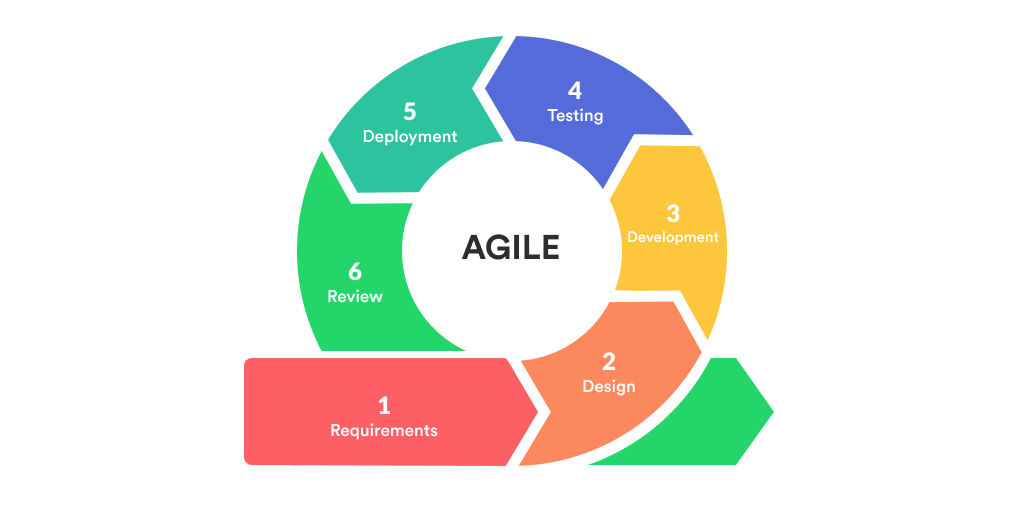
\includegraphics[totalheight=8cm]{Introduction/AgileModel.png}
    \caption{Software Development Life Cycle Model}
    \label{fig:verticalcell}
\end{figure}


\section{Organization of Report}
% Content inside the organization of the report goes here

Chapter 1: Chapter 1, Problem definition of the proposed machine learning model is given along with background history, motivation for developing this system. Scope and objective of projected system is discussed.\\ 
Chapter 2: Chapter 2, will talk about literature referred for getting this idea of project design. Actual working and functionalities of the proposed machine learning model is described here. Section 2.1 will be brief about economical, operational and technical feasibility of the given system. Risk analysis is done in section 2.2 along with planning and effort allocation for development of proposed system in section 2.3 and 2.4.\\
Chapter 3: Chapter 3, will discuss about requirements of machine learning model. Hardware as well as software requirements are described in section 3.1 and section 3.2. Section 3.3 will give functional and non functional requirements of the the model. And software requirements specification is stated in section 3.4.\\
Chapter 4: Chapter 4 will give pictorial representation of the system. Section 4.1 will show architecture of the machine learning model using simple block diagram. Section 4.2 will give data flow diagrams (DFDs). UML diagrams of the proposed system are given in section 4.3.\\
Chapter 5: In chapter 5, conclusion about whatever work had done is discussed in section 5.1. Future work are discussed in section 5.2. At the last, project report embody bibliography too.


\section{Summary}
% Content of the summary section goes here
The given chapter thoroughly describes background and motivation behind selecting this machine learning project. The problem definition, scope and objective are also stated in the given chapter. The organization of report gave the overall structure about the chapters described throughout in this report upfront. The next chapter will discuss about system analysis.


\chapter{Project Planning and Management}
Requirements analysis is a software engineering task that has bridged the gap between system level requirements engineering and software design requirement engineering activities resulting in the specification of software’s operational characteristics (functional, data, and behavioral), that indicates software’s interface with other system elements and establishes constraints that software must meet. Gathering of requirements related to the proposed system is done. Analysis is done by comparing these requirements with working and function provided by ’existing forum system’.\\ The proposed chapter will discuss about feasibility study of the proposed system in section 2.1. The section 2.2 discuss about risk analysis. The project scheduling of system is described in section 2.3. The section 2.4 will discuss about effort allocation. Cost estimation is discussed in section 2.5. Finally the summary in last section.

\section{Feasibility Study}
% Content inside the feasibility study goes here

While considering the feasibility of any system, the system must meet its best performance by three sides i.e. technical, operational and economical feasibility. Feasibility should be considered in any organization since it helps in selection of best system for the job. It is necessary to evaluate the feasibility of the project at the early stages of software development.\\
\textbf{If project risk is great, the feasibility of product is reduced.}\\
A well designed feasibility study should provide a description of the product or service, details
of operation and working of system. A feasibility study evaluates the project potential for
success; The types of feasibility study are:
    \subsection{Technical Feasibility}
    \subsection{Operational Feasibility}
    \subsection{Economical Feasibility}

\section{Risk Analysis}
% Content if the risk analysis goes here

Risk analysis and management are actions that help a software team to understand and
manage uncertainty. A risk is a potential problem it might happen, or it may not. Risk is a uncertain event or condition that, if it occurs, has a positive or negative effect on a project’s objectives.\\
Risk always involves two characteristics: \textbf{uncertainty}- the risk may or may not happen; that is, there are no 100 percent probable risk and \textbf{loss}- if the risk becomes a reality ,unwanted consequences or losses will occur. When risks are analyzed, it is important to quantify the level of uncertainty and the degree of loss associated with each risk. The different types of risks are-\\

\begin{itemize}
    
    \item \textbf{Project Risk} threaten the project plan. That is, if project risks become real, it is likely that the project schedule will slip and that cost will increase. Project risk identify potential budgetary, schedule, personnel, resource, stakeholder, and requirements problems and their impact on a software etc.

    \item \textbf{Technical Risk} threaten the project plan. That is, if project risks become real, it is likely that the project schedule will slip and that cost will increase. Project risk identify potential budgetary, schedule, personnel, resource, stakeholder, and requirements problems and their impact on a software etc.

    
    \item \textbf{Business Risk} threaten the viability of software to be built and often jeopardize the project or the product. Candidates for the top five business risks are:
    
        \begin{enumerate}
            \item Building an excellent product or system that no one really wants\textbf{(market risk)}.
            \item Building a product that no longer fits into overall business strategy for the company\textbf{(strategic risk)}.
            \item Building a product that the sales force doesn’t understand how to sell\textbf{(sale risk)}.
            \item Losing the support of senior management due to a change in focus or a change in people\textbf{(management risk)}.
            \item  Losing budget or personnel commitment\textbf{(budget risks)}.
    
        \end{enumerate}
        
\end{itemize}
% some space is remaining herre

% Risk Analysis Table >>>>>>>>>>>
\newpage
\begin{table}[!ht]
\centering
\begin{tabular}{|l|l|l|l|}
\hline
Risk                                  & Category & Probability & Impact \\ \hline
Technology will not meet requirements & TE       & 30\%        & 1      \\ \hline
End-user resist the system            & BU       & 40\%        & 3      \\ \hline
\end{tabular}
\caption{Risk Analysis}
\end{table}

\begin{enumerate}
    \item \textbf{Catastrophic}: Failure to meet requirement would result in mission failure or increase in cost which includes schedule delay.
    \item \textbf{Critical}: Some reduction in technical performance.
    \item \textbf{Marginal}: Minimal to small reduction in technical performance.
    \item \textbf{Negligible}: No reduction in technical performance.

\end{enumerate}


\section{Project Scheduling}
\begin{figure}[h]
    \centering
    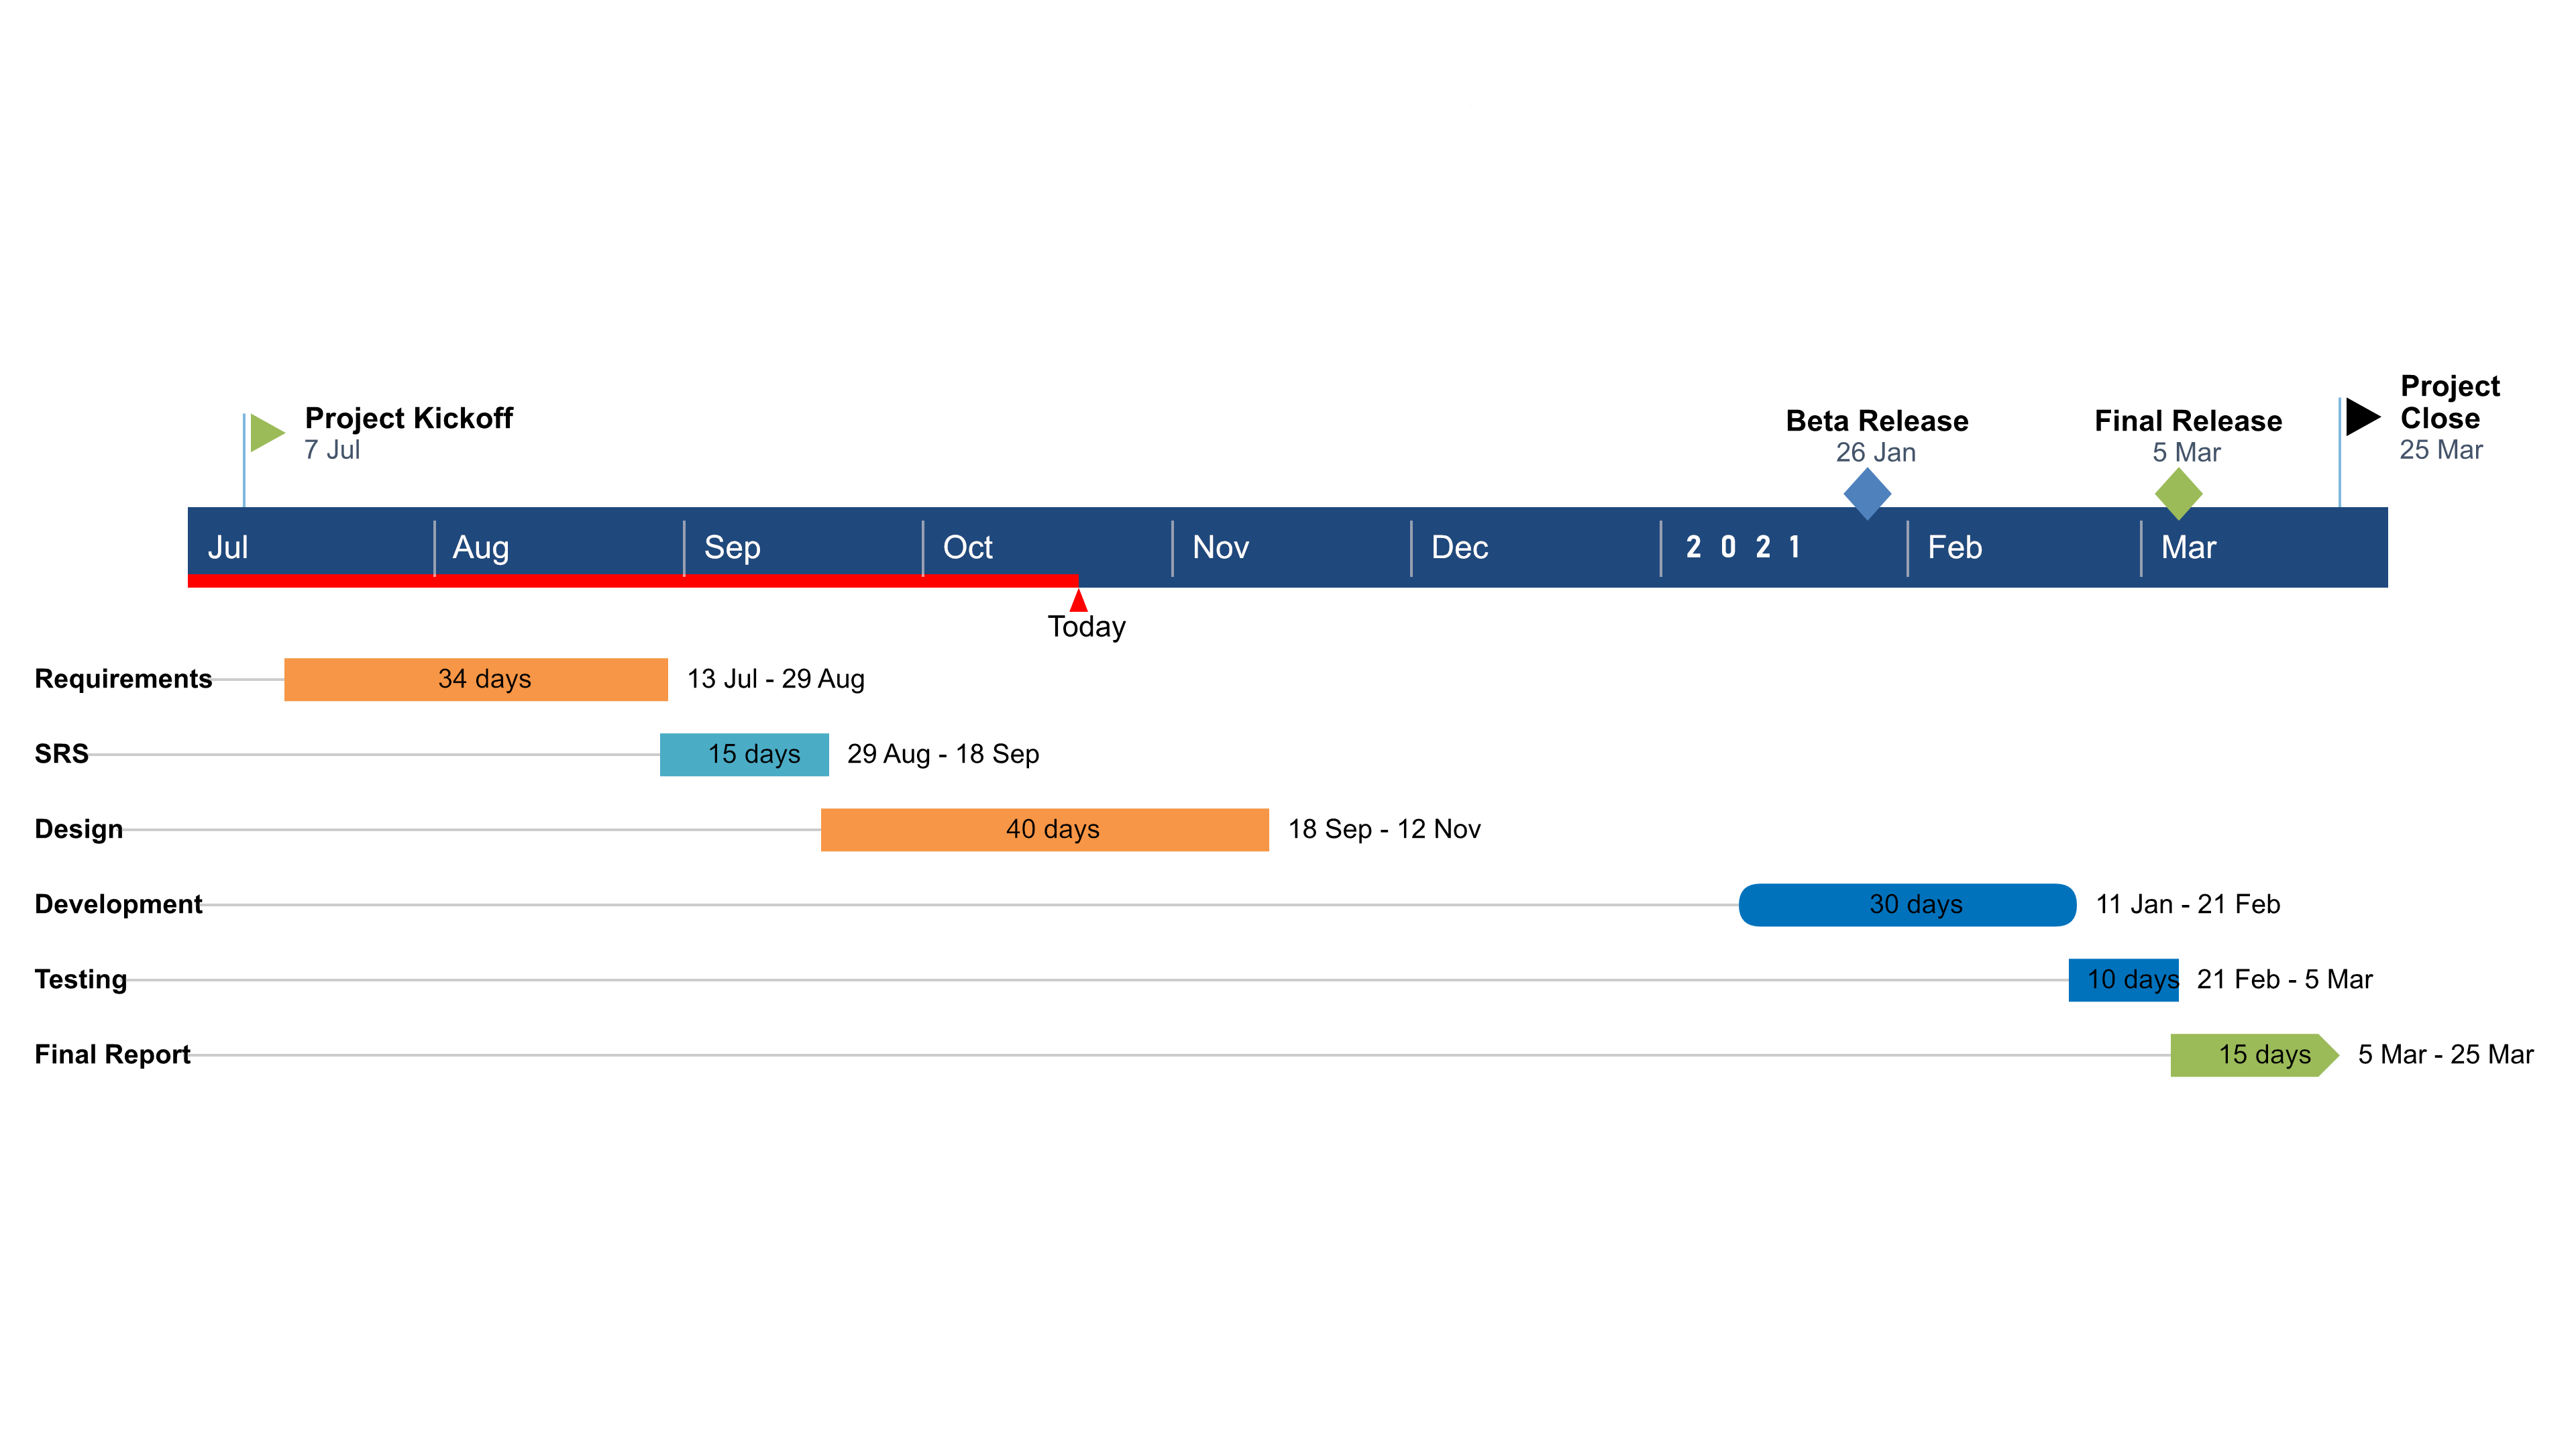
\includegraphics[width=\textwidth]{Project Planning and Management/Gantt_char_new.png}
    \caption{Gantt Chart}
    % \label{fig:my_label}
\end{figure}
\newpage

\section{Effort Allocation}
\begin{figure}[!ht]
    \centering
    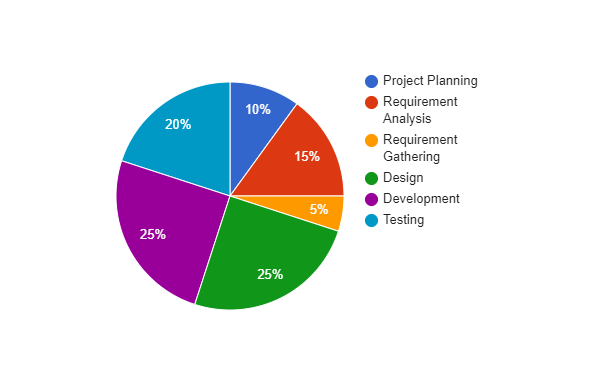
\includegraphics[width=\textwidth]{Project Planning and Management/Effort Allocation.png}
    \caption{Effort Allocation}
    \label{fig:my_label}
\end{figure}
    

\section{Cost Estimation}
    \subsection{COCOMO Model}

\section{Summary}
% Content of the summary goes here
The given chapter thoroughly describes feasibility study, risk analysis, project scheduling, effort allocation and cost estimation. The next chapter will discuss about analysis.


\chapter{Analysis}
Requirements analysis is a software engineering task that bridges the gap between system level requirements engineering and software design Requirement engineering activities result in the specification of software’s operational characteristics (functional, data, and behavioral), indicate software’s interface with other system elements, and establish constraints that software must meet.\\
The chapter contains system requirements of the proposed system. The requirement collection and identification of propose system are described in section 3.1. The section 3.2 will discuss about hardware and software requirements of system. In Section 3.3 functional and non functional requirements of proposed system will be discussed. The software requirement’s specification of system will be discussed in section 3.4. Finally the summary in last section.

\section{Requirement Collection and Identification}
\section{Software Requirement Specification}
    \subsection{Product Features}
    \subsection{Operating Environment}
    \subsection{Assumptions}
    \subsection{Functional Requirements}
    \subsection{Non-Functional Requirements}
    \subsection{External Interfaces (User, Hardware, Software, Communication)}

\section{Summary}
In this chapter all the system requirements specification is described. System design will be discussed in next chapter.


\chapter{System Design}
Design is a meaningful engineering representation of something that is to be built. It can be traced to system requirements and at the same time assessed for quality against a set of predefined criteria for ”good” design. Software design sits at the technical kernel of software
engineering and is applied regardless of software process model that is used. Software design is the first of three technical activities-design, code generation and test that are required to build and verify the software.\\
The respective chapter will discuss about the proposed system design. Section 4.1 will discuss about the system architecture. Data Flow Diagram’s are discussed in section 4.2. Section 4.3 contains the UML diagrams. Finally the summary in last section.

\section{System Architecture}
\section{Data Flow Diagrams}
    \subsection{Level 0 DFD}
    \subsection{Level 1 DFD}
\section{UML Diagrams}
    \subsection{Use Case Diagram}
    \subsection{Class Diagram}
    \subsection{Sequence Diagram}
    \subsection{Component Diagram}
    \subsection{Deployment Diagram}
    \subsection{State Chart Diagram}
    \subsection{Activity Diagram}

\section{Summary}
% Content of the summary goes here
The given chapter thoroughly describes system design. The next chapter will discuss about conclusion and future work.


\chapter{Conclusion and Future Work}
\section{Conclusion}
\section{Future Work}




\printindex

\end{document}
